
\documentclass[10pt]{SelfArx} % Document font size and equations flushed left

\usepackage[english]{babel} % Specify a different language here - english by default




% Default fixed font does not support bold face
\DeclareFixedFont{\ttb}{T1}{txtt}{bx}{n}{12} % for bold
\DeclareFixedFont{\ttm}{T1}{txtt}{m}{n}{12}  % for normal

% Custom colors
\usepackage{color}
\definecolor{deepblue}{rgb}{0,0,0.5}
\definecolor{deepred}{rgb}{0.6,0,0}
\definecolor{deepgreen}{rgb}{0,0.5,0}

\usepackage{listings}
 \usepackage{booktabs}
 
% Python style for highlighting
\newcommand\pythonstyle{\lstset{
		language=Python,
		basicstyle=\ttm,
		otherkeywords={self},             % Add keywords here
		keywordstyle=\ttb\color{deepblue},
		emph={MyClass,__init__},          % Custom highlighting
		emphstyle=\ttb\color{deepred},    % Custom highlighting style
		stringstyle=\color{deepgreen},
		frame=tb,                         % Any extra options here
		showstringspaces=false            % 
}}


% Python environment
\lstnewenvironment{python}[1][]
{
	\pythonstyle
	\lstset{#1}
}
{}

% Python for external files
\newcommand\pythonexternal[2][]{{
		\pythonstyle
		\lstinputlisting[#1]{#2}}}

% Python for inline
\newcommand\pythoninline[1]{{\pythonstyle\lstinline!#1!}}

%----------------------------------------------------------------------------------------
%	COLUMNS
%----------------------------------------------------------------------------------------

\setlength{\columnsep}{0.55cm} % Distance between the two columns of text
\setlength{\fboxrule}{0.75pt} % Width of the border around the abstract

%----------------------------------------------------------------------------------------
%	COLORS
%----------------------------------------------------------------------------------------

\definecolor{color1}{RGB}{0,0,90} % Color of the article title and sections
\definecolor{color2}{RGB}{0,20,20} % Color of the boxes behind the abstract and headings

%----------------------------------------------------------------------------------------
%	HYPERLINKS
%----------------------------------------------------------------------------------------

\usepackage{hyperref} % Required for hyperlinks
\hypersetup{hidelinks,colorlinks,breaklinks=true,urlcolor=color2,citecolor=color1,linkcolor=color1,bookmarksopen=false,pdftitle={Title},pdfauthor={Author}}

%----------------------------------------------------------------------------------------
%	ARTICLE INFORMATION
%----------------------------------------------------------------------------------------

\JournalInfo{Nov 23, 2019}
\Archive{Shahid Beheshti University}

\PaperTitle{Implementing deep neural networks for classification and regression tasks}

\Authors{Alireza Afzal Aghaei\textsuperscript{1}*}
\affiliation{\textsuperscript{1}\textit{Department of Computer Science, Shahid Beheshti University, Tehran, Iran}} \affiliation{*\textbf{Corresponding author}: alirezaafzalaghaei@gmail.com}

\Keywords{Deep learning, Convolutional neural networks, Recurrent neural networks} % Keywords - if you don't want any simply remove all the text between the curly brackets
\newcommand{\keywordname}{Keywords} % Defines the keywords heading name

%----------------------------------------------------------------------------------------
%	ABSTRACT
%----------------------------------------------------------------------------------------

\Abstract{
In this report, we explain the mathematics behind deep neural networks by starting from multi layer perceptron (MLP) model, then discuss convolutional neural networks (CNN) and recurrent neural networks (RNN). To increase generalization of the models we explained weight regularization method as a powerful method among regularization techniques. To show the accuracy of models we use some datasets for classification tasks on iris dataset. then used CNN model on mnist and fashion mnist dataset and finally applied RNNs on sentiment analysis task.
}

%----------------------------------------------------------------------------------------

\begin{document}

\flushbottom % Makes all text pages the same height

\maketitle % Print the title and abstract box
\tableofcontents % Print the contents section

\thispagestyle{empty} % Removes page numbering from the first page

%----------------------------------------------------------------------------------------
%	ARTICLE CONTENTS
%----------------------------------------------------------------------------------------

\section*{Introduction} % The \section*{} command stops section numbering

\addcontentsline{toc}{section}{Introduction} % Adds this section to the table of contents
ANNs began as an attempt to exploit the architecture of the human brain to perform tasks that conventional algorithms had little success with. They retained the biological concept of artificial neurons, which receive input, combine the input with their internal state (activation) and an optional threshold using an activation function, and produce output using an output function. The initial inputs are external data, such as images and documents. The ultimate outputs accomplish the task, such as recognizing an object in an image. The important characteristic of the activation function is that it provides a smooth transition as input values change, i.e. a small change in input produces a small change in output.The network consists of connections, each connection providing the output of one neuron as an input to another neuron. Each connection is assigned a weight that represents its relative importance. A given neuron can have multiple input and output connections.
\begin{figure}\centering
			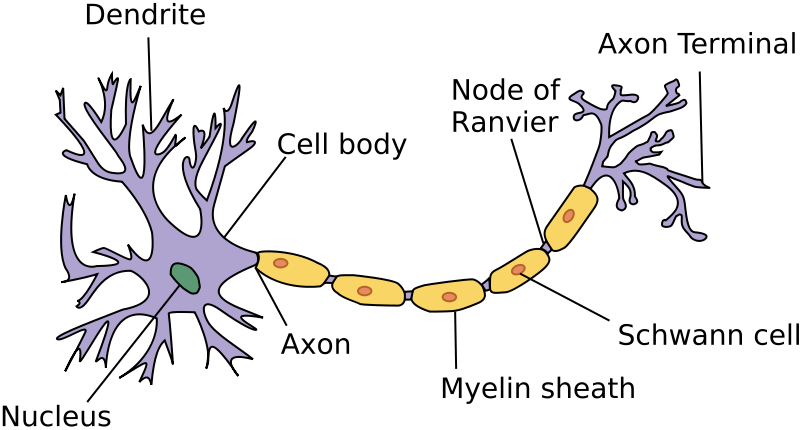
\includegraphics[width=\linewidth]{img/neuron}
	\caption{A biological neuron}
		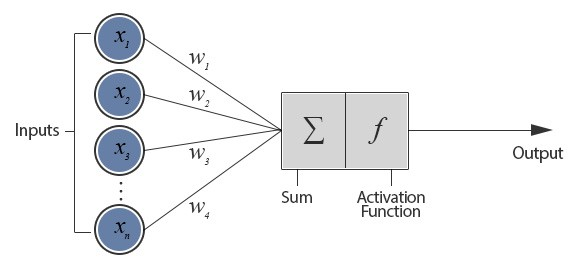
\includegraphics[width=\linewidth]{img/aneuron}
	\caption{An artificial neuron}	
\end{figure}
A biological neuron made of a cell body (Soma), dendrites and an axon. Dendrite receives signals from other neurons, Soma sums all the incoming signals to generate input, Axon fires when the sum reaches a threshold value and sends a signal to the synapse where is the point of interconnection of one neuron with other neurons.


%\begin{figure}\centering % Using \begin{figure*} makes the figure take up the entire width of the page
%
%\end{figure}

Artificial neuron simulates the structure of a biological neuron. As of the simplicity of derivative calculation, it uses sum of product of input and corresponding weights. It fires, if the summation reaches to a threshold. Note that, because of good approximation of fuzzy activation functions, the function $f$ maybe more complex than simple threshold function. This functions should be continuous and (weakly) differentiable. For example, $Tanh$, $Relu$ and its variants, $Sigmoid$ and radial basis functions ($RBFs$) are some of them. Same as linear regression, by finding set of appropriate weights, we can solve a linear regression problem with this approach.

\begin{figure}\centering % Using \begin{figure*} makes the figure take up the entire width of the page
	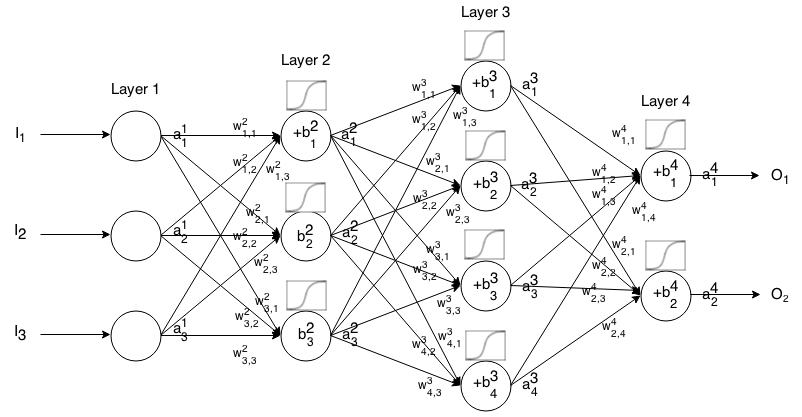
\includegraphics[width=\linewidth]{img/ann}
	\caption{An Artificial neural network}	
\end{figure}

An artificial neural network (ANN) consist of many single neurons connected to each other with a specific structure. Multi layer perceptron (MLP) is a most basic network which neurons are stacked in several layers. Convolutional and recurrent neural networks are other types of ANNs. By training a network we can find optimal weights which leads to a good approximation of desired dataset. This process can be divided into three major phases:
Forward pass, Backward pass and, Updating weights. In the two next Sections we explain mathematics behind state-of-the-art networks such as MLP and CNN which can be trained using backpropagation algorithm and gradient descent optimizer for supervised tasks.


%------------------------------------------------

\section{Multi layer perceptron (MLP)}
In this section, we explain backpropagation algorithm for MLP networks and introduce some activation and loss functions which are used for classification and regression tasks. 

\subsection{Forward phase}
Suppose a $d$-dimensional dataset contains $n$ different samples named $X^{n\times d}$ and $k$-dimensional target values $Y^{n\times k}$. By defining a weight matrix $W_{1}^{d\times h1}$ and using matrix multiplication we have
\begin{equation}
z^{(1)} = X \cdot W_1
\end{equation}
which $Z^{(1)}$ denotes first hidden layer of network. This process is equal to apply simple weighted summation for whole dataset. By applying a nonlinear activation function we have
\begin{equation}
a^{(1)} = \sigma(z^{(1)}).
\end{equation}

It's clear that the shape of $a^{(1)}$ is $(n \times h1)$. We can repeat this process to build deeper network.
\begin{equation}
z^{(i)} = a^{(i-1)} \cdot W_i 
\end{equation}
\begin{equation}
a^{(i)} = \sigma(z^{(i)})
\end{equation}
for $i=2,\ldots,r-1$. In the last layer, we have
\begin{equation}
z^{(r)} = a^{(r-1)} \cdot W_r
\end{equation}
\begin{equation}
\hat{y} = \sigma(Z^{(r)})
\end{equation}
which $\hat{y}$ is the prediction of neural network w.r.t input data $X$ and weights $\{W_i\}_{i=1}^r$.

\subsection{Loss function}
To see the accuracy of the network, we need a measure function to show the cost of prediction. The most known loss functions are mean squared error (MSE) end cross entropy (Xentropy) which are used in regression and classifications tasks, respectively. There are many other loss functions such as mean absolute error, Vapnik's $\epsilon$-insensitive loss function, etc. Here we explain MSE loss function:
\begin{equation}
J_{MSE}(W) ={\frac {1}{n}}\sum\limits_{i=1}^{n}(y_{i}-{\hat {y_{i}}})^{2}
\end{equation}

\subsection{Backward phase: Backpropagation}
To find optimal weights with mathematics optimization tools, we need the derivative of loss function w.r.t weights $W_{i,j}^r$. Here we provide a well known technique known as Backpropagation.
by defining
\begin{equation}
\delta^{(l)} = -(y - a^{(l)})\odot\sigma'(z^{(l)})
\end{equation}
For last layer and 
\begin{equation}
\delta^{(l)} = (\delta^{(l + 1)} \cdot W_{l}^{\intercal})\odot\sigma'(z^{(l)})
\end{equation}
the derivatives can be computed by
\begin{equation}
\displaystyle\frac{\partial J(W)}{\partial W_{l}} = a^{(l)\intercal} \cdot \delta^{(l + 1)}
\end{equation}
For better explanation see \href{https://brilliant.org/wiki/backpropagation/}{Brilliant backpropagation tutorial}

\subsection{Update phase}
\begin{figure}\centering 
	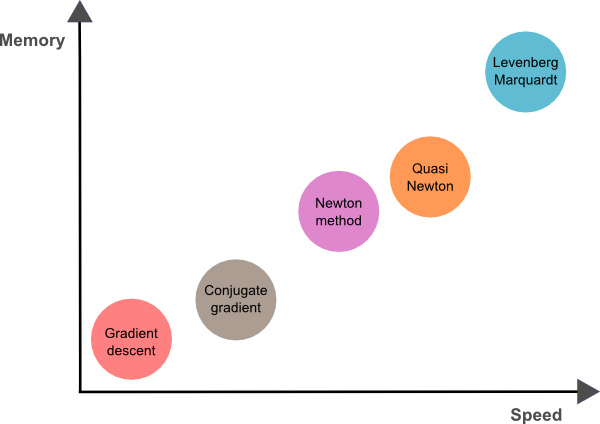
\includegraphics[width=\linewidth]{img/optimizer}
	\caption{Different optimizers}
\end{figure}
Function minimization is an essential topic in mathematics. When the function $f(x)$ has quadratic form, there is special optimizer which can rich global minimum efficiently. But for arbitrary nonlinear functions we need to use some parametric iterative algorithms to reach the a minimum point that maybe is a local. Based of the derivative order needed by algorithms the classified into two categories known as first and second order methods. While first order methods need to save gradient vector in memory, second order optimizers save a matrix of derivatives. Since these methods are very memory intensive for large datasets, some algorithms are developed which approximate that matrix among gradient calculation. The most known algorithms is Limited memory-BFGS (L-BFGS). Because of simple implementation, here we explain gradient descent algorithm which is a very basic first order optimizer.
By starting from an initial point $w_0$ and goal function $L$, we can reach a local minimum with this update rule:
\begin{equation}
w_i = w_i - \eta \frac{\partial L}{\partial w_i}
\end{equation}
where $\eta$ called step length or learning rate. Note that, by choosing appropriate value for step length we can reach global minimum. To accelerate the learning process, researchers extended this update rule by adding some terms or changing step length base on some conditions. Momentom, Nestrov, Adagrad, AdaDelta, RMSProp, Adam are some extensions of vanilla gradient descent. see \href{https://ruder.io/optimizing-gradient-descent/}{ruder.io} for better formulation and pseudo-codes.

\subsection{Weight regularization}
There are several techniques which are used overcome the over-fitting problem. Among them weight decay and dropout are major methods. In weight decay, we add a positive function of unknown weights to the loss function. This leads to small weights and help us to prevent over-fitting. because of simplicity here we explain L2-regularization which is named as Tikhonov regularization in mathematics.
This regularization, can be defined by adding 
\begin{equation}
\centering
\alpha \sum_{i=1}^r \Vert W_i \Vert_F
\end{equation}
term to the loss function, where $\Vert \cdot \Vert_F$ denotes Frobinious norm and $\alpha$ is the regularization coefficient.
\subsection{Dropout}
Dropout is a regularization technique for reducing overfitting in neural networks by preventing complex co-adaptations on training data. It is a very efficient way of performing model averaging with neural networks. The term "dropout" refers to dropping out units (both hidden and visible) in a neural network.
\section{Convolutional neural network (CNN)}
In this section we introduce convolution and pooling operators used in Convolutional neural networks. Then derive the backpropagation formulas for these operators. 
\subsection{Convolution and Pooling block}
\begin{figure}\centering 
	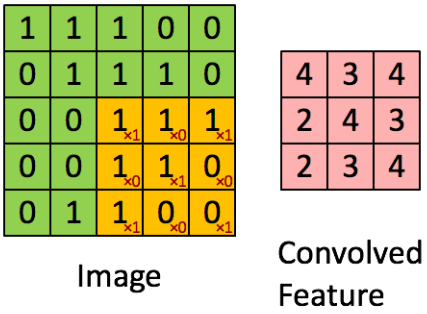
\includegraphics[width=.6\linewidth]{img/conv}
	\caption{Convolution operator}		
	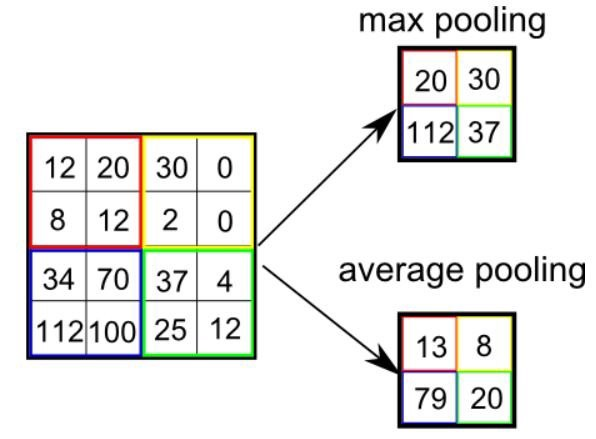
\includegraphics[width=.6\linewidth]{img/pooling}
	\caption{Pooling layer}	
\end{figure}
The objective of the Convolution Operation is to extract the high-level features such as edges, from the input image. ConvNets need not be limited to only one Convolutional Layer. Conventionally, the first ConvLayer is responsible for capturing the Low-Level features such as edges, color, gradient orientation, etc. With added layers, the architecture adapts to the High-Level features as well, giving us a network which has the wholesome understanding of images in the dataset, similar to how we would.
There are two types of results to the operation — one in which the convolved feature is reduced in dimensionality as compared to the input, and the other in which the dimensionality is either increased or remains the same. This is done by applying Valid Padding in case of the former, or Same Padding in the case of the latter.

Similar to the Convolutional Layer, the Pooling layer is responsible for reducing the spatial size of the Convolved Feature. This is to decrease the computational power required to process the data through dimensionality reduction. Furthermore, it is useful for extracting dominant features which are rotational and positional invariant, thus maintaining the process of effectively training of the model.
There are two types of Pooling: Max Pooling and Average Pooling. Max Pooling returns the maximum value from the portion of the image covered by the Kernel. On the other hand, Average Pooling returns the average of all the values from the portion of the image covered by the Kernel.
Max Pooling also performs as a Noise Suppressant. It discards the noisy activations altogether and also performs de-noising along with dimensionality reduction. On the other hand, Average Pooling simply performs dimensionality reduction as a noise suppressing mechanism. Hence, we can say that Max Pooling performs a lot better than Average Pooling.

The Convolutional Layer and the Pooling Layer, together form the i-th layer of a Convolutional Neural Network. Depending on the complexities in the images, the number of such layers may be increased for capturing low-levels details even further, but at the cost of more computational power.
After going through the above process, we have successfully enabled the model to understand the features. Moving on, we are going to flatten the final output and feed it to a regular Neural Network for classification purposes.
\subsection{Backward phase}
See \href{https://medium.com/@2017csm1006/forward-and-backpropagation-in-convolutional-neural-network-4dfa96d7b37e}{this} and \href{https://becominghuman.ai/back-propagation-in-convolutional-neural-networks-intuition-and-code-714ef1c38199}{this} for backward phase of convolution and pooling layers.

\section{Recurrent neural network (RNN)}
A recurrent neural network (RNN) is a class of artificial neural networks where connections between nodes form a directed graph along a temporal sequence. This allows it to exhibit temporal dynamic behavior. Unlike feedforward neural networks, RNNs can use their internal state (memory) to process sequences of inputs. This makes them applicable to tasks such as unsegmented, connected handwriting recognition or speech recognition.
\begin{figure}\centering 
	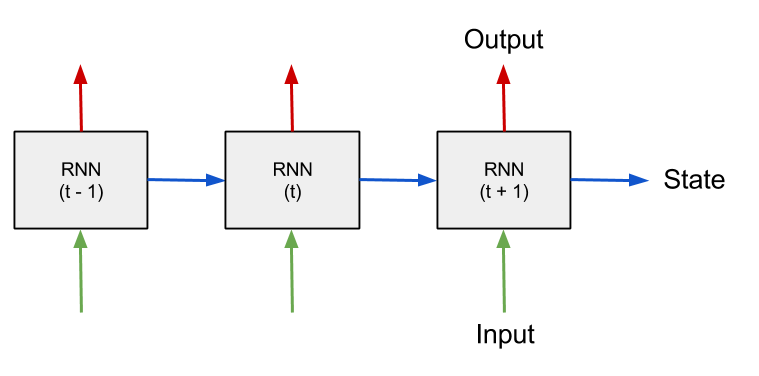
\includegraphics[width=.6\linewidth]{img/rnn}
	\caption{RNN}
\end{figure}
\subsection{LSTM}
A common LSTM unit is composed of a cell, an input gate, an output gate and a forget gate. The cell remembers values over arbitrary time intervals and the three gates regulate the flow of information into and out of the cell.
\begin{figure}\centering 
	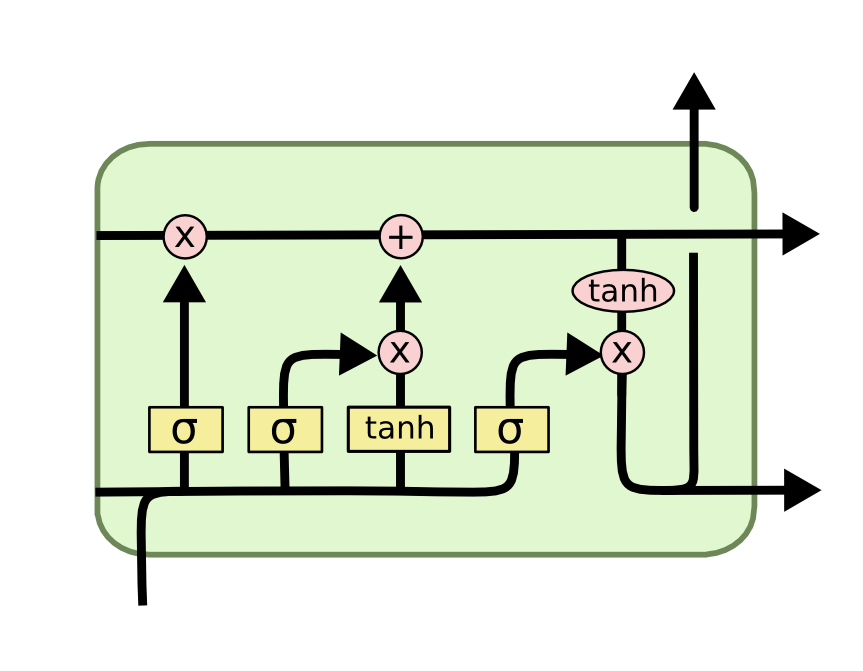
\includegraphics[width=.6\linewidth]{img/lstm}
	\caption{LSTM cell}
\end{figure}
\subsection{GRU}
The GRU is like a long short-term memory (LSTM) with forget gate[2] but has fewer parameters than LSTM, as it lacks an output gate. GRU's performance on certain tasks of polyphonic music modeling and speech signal modeling was found to be similar to that of LSTM. GRUs have been shown to exhibit even better performance on certain smaller datasets. However, as shown by Gail Weiss \& Yoav Goldberg \& Eran Yahav, the LSTM is "strictly stronger" than the GRU as it can easily perform unbounded counting, while the GRU cannot.That's why the GRU fails to learn simple languages that are learnable by the LSTM. 
\subsection{Backward phase}
The error backpropagation algorithm for recurrent networks is named as backpropagation trough time (BPTT). see  \href{https://machinelearningmastery.com/gentle-introduction-backpropagation-time/}{this link} for more information about BTPP.
\section{Text analysis}
\subsection{Embedding}
Word embedding is a technique used to represent documents with a dense vector representation. The vocabulary in these documents is mapped to real number vectors. Words that are semantically similar are mapped close to each other in the vector space. 

%------------------------------------------------

\section{Implementation}

In all of the examples for MLP training, we first normalize input data by subtracting mean of a column for each data sample then dividing it by variance of column. In the regression datasets, we do the same scaling on target values, but in the classification tasks, one-hot encoding is used.
This process is done automatically by following implemented class.

\subsection{MLP model}

The implementation of our MLP class is defind as a simple class named MLP.

\begin{python}
MLP(hidden_layer, activation,
    epoch, eta, beta, alpha, mu,
    batch_size, verbose, task)
\end{python}
where options are
\begin{itemize}
\item \textbf{hidden\_layer}: A list where each item defines the number of neurons in the hidden layer. It's obvious that, the length of list denotes number of hidden layers.
\item \textbf{activation}: A single class that inherits Activation class and applied to each layer. Default choices are Sigmoid, Tanh, ReLU and LeakyReLU.
\item \textbf{epoch}: The number of iterations.
\item \textbf{eta}: Step length or learning rate
\item \textbf{beta}: A number which multiplied to initial weights, initial weights have normal distribution
\item \textbf{alpha}: Regularization coefficient
\item \textbf{mu}: Momentum parameter
\item \textbf{batch\_size}: The number of batch passed to batch gradient descent
\item \textbf{verbose}: (optional) Use this to show the loss of i-th iteration.

\item \textbf{task}: Must be one of regression or classification. Based on task, this class encodes output values and also chooses activation function of last layer automatically.
\end{itemize}
This class implements this methods:
\begin{itemize}
\item  \textbf{fit(x\_train, y\_train, validation: optional = list(x\_valid, y\_valid))}
\item  \textbf{predict(x)}
\item  \textbf{score(x,y)
}
\end{itemize}
fit function returns the pair (history, validation\_history) if the validation set was set. Otherwise it returns history of training phase. Each of these, contains a 2d numpy array with the shape of (n\_iterations, 2). The columns contain loss and score history during training phase, respectively.
predict function returns the predicted values for input x.
score functions returns the score of model with input x and output y. This function uses accuracy\_score and r2\_score metrics implemented in scikit-learn module for classification and regression tasks.


\subsection{CNN Model}
For this case we used keras API and implemented a simple class to be compatible with previous MLP class.
\begin{python}
CNN(architecture, epochs,
   batch_size, optimizer, loss,
   metrics, task, verbose)
\end{python}
where arguments are
\begin{itemize}
\item 	\textbf{architecture}: list of keras layers such as Cond2D, Dense, etc.
\item  \textbf{epochs}: number of epochs
\item  \textbf{batch\_size}: size of the batch for gradient descent optimizer
\item  \textbf{optimizer}: keras optimizer such as adam or sgd
\item  \textbf{loss}: loss function, same as keras loss functions
\item \textbf{metrics}: list of metrics, same as keras
\item  \textbf{task}: regression or classification
\item  \textbf{verbose}: print training information, same as keras
\end{itemize}

same as MLP model, this class implements three methods fit, score and predict. everything is same as previous one except fit function which gets some keyword arguments and pass them to keras fit function. So use keras validation\_data to validate model on specific data.

\subsection{RNN Model}
Again, For this case we used keras API and implemented a simple class to be compatible with previous both MLP and CNN class.
\begin{python}
	RNN(architecture, epochs,
	batch_size, optimizer, loss,
	metrics, task, verbose)
\end{python}
where arguments are
\begin{itemize}
	\item 	\textbf{architecture}: list of keras layers such as LSTM, Dense, etc.
	\item  \textbf{epochs}: number of epochs
	\item  \textbf{batch\_size}: size of the batch for gradient descent optimizer
	\item  \textbf{optimizer}: keras optimizer such as adam or sgd
	\item  \textbf{loss}: loss function, same as keras loss functions
	\item \textbf{metrics}: list of metrics, same as keras
	\item  \textbf{task}: regression or classification
	\item  \textbf{verbose}: print training information, same as keras
\end{itemize}

same as CNN model, this class implements three methods fit, score and predict.

\subsection{Hyperparameter tuning}
To find optimal architecture of network, grid search is a simple and efficient way. By passing a set of different possible choices for a problem, the following classes run and save all possible architectures and their corresponding loss history.
\begin{python}
MLPGridSearch(task, hidden_layers, 
      activations batch_sizes,
      epochs, mus, betas, etas,
      alphas, filename)
\end{python}
for CNN
\begin{python}
CNNGridSearch(architecture,epochs,
	  batch_sizes, optimizers,
	  file_name)
\end{python}
and RNN
\begin{python}
RNNGridSearch(architecture,epochs,
batch_sizes, optimizers,
file_name)
\end{python}

These classes implement two methods run and best\_model which return history of models and the best model which has best accuracy and lower loss, respectively. Also a parallelization technique for multi-core processors has been implemented on MLPGridSearch class to speedup searching process. Because of GPU limitations we cannot implement parallelization on CNNGridSearch and RNNGridSearch.

\section{Results and Discussion}

\subsection{Iris}
Dataset description:
\begin{itemize}
	\item Input data: 4 features of 150 iris flowers
	
	\item Target value: 3 different type of iris	
	
	\item \href{https://archive.ics.uci.edu/ml/datasets/Iris}{More information in UCI repository}
\end{itemize}
The grid search parameters were set to:
\begin{python}
hidden_layers = [(5, 5, 5, 5),
(10, 10, 5),(15, 15),(20, 15, 10),
       (32,)]
activations = [Tanh(), ReLu(),
                LeakyReLu(.1)]
batch_sizes = [16, 64, 128]
epochs = [300]
mus = [0, .8]
betas = [.3]
etas = [.01, 0.001]
alphas = [.001, .01, 0]
\end{python}
See the results in the table \ref{tiris}. In this example, we saw that:
\begin{itemize}
\item  LeakyReLu acts like Relu function in some situations.
\item  Maybe test accuracy becomes better that train accuracy.
\item  Momentum technique plays an important role in optimization path. All of 6 best architectures are using momentum.
\item  Choosing learning is tricky and help us to reach global minimum in less epochs. By choosing big values for learning rate, the training phase becomes unstable and the MLP class raises floating point overflow.
\item  Smaller batch size help us to reach minimum faster.
\end{itemize}
\begin{table*}[hbt]
	\centering
  \begin{tabular*}{1\textwidth}{@{\extracolsep{\fill} }ccccccccccc@{}}
	\toprule
	hidden\_layer & activation & epoch & eta & beta & alpha & mu & batch\_size & test\_score & train\_score & loss \\ \midrule
	(10, 10, 5) & ReLu & 300 & 0.01 & 0.3 & 0.01 & 0.8 & 16 & 1.00 & 0.97 & 0.84 \\
	(10, 10, 5) & LeakyReLu(0.1) & 300 & 0.01 & 0.3 & 0.01 & 0.8 & 16 & 1.00 & 0.96 & 1.28 \\
	(15, 15) & Tanh & 300 & 0.01 & 0.3 & 0.01 & 0.8 & 16 & 0.97 & 0.98 & 0.67 \\
	(5, 5, 5, 5) & ReLu & 300 & 0.01 & 0.3 & 0.01 & 0.8 & 16 & 0.97 & 0.97 & 0.85 \\
	(15, 15) & ReLu & 300 & 0.01 & 0.3 & 0.01 & 0.8 & 16 & 0.97 & 0.97 & 0.87 \\ \bottomrule
\end{tabular*}
	\captionof{table}{Best architectures and corresponding scores for IRIS dataset}
	\label{tiris}
\end{table*}
\begin{figure*}\centering
	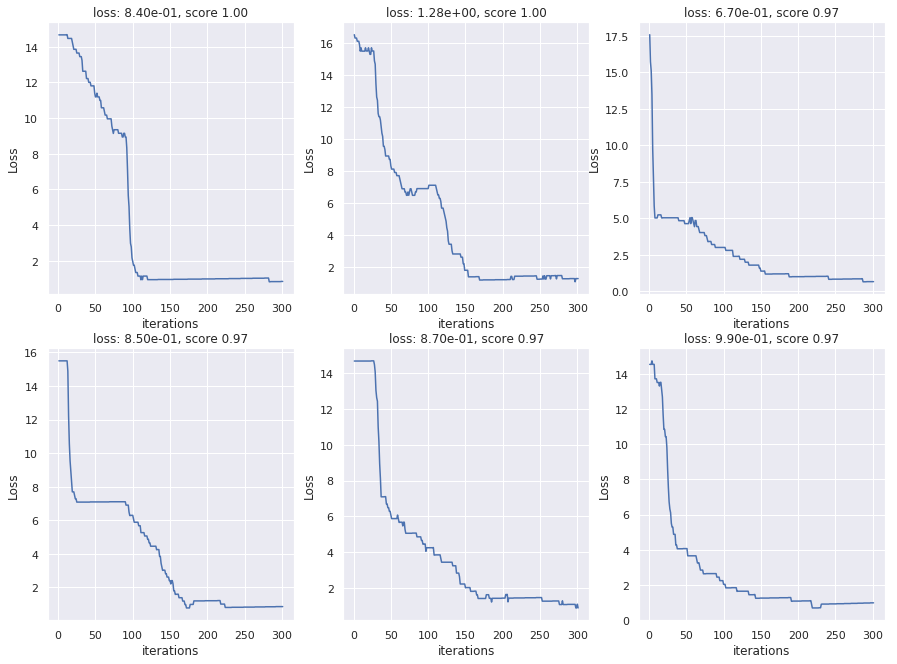
\includegraphics[width=1.79\columnwidth, height=10cm]{img/iris-plots1}
	\caption{Loss value of best architectures for IRIS}
	\label{firis}
\end{figure*}

\subsection{Statlog}
The database consists of the multi-spectral values of pixels in 3x3 neighborhoods in a satellite image, and the classification associated with the central pixel in each neighborhood. The aim is to predict this classification, given the multi-spectral values. In the sample database, the class of a pixel is coded as a number. \href{https://archive.ics.uci.edu/ml/datasets/Statlog+(Landsat+Satellite)}{More information about this dataset is available in UCI repository.}

The grid search parameters is set to

\begin{python}
hidden_layers = [(32, 16, 8),
             (10, 10, 10), (64,)]
activations = [Tanh(), Sigmoid(),
               ReLu()]
batch_sizes = [256]
epochs = [30]
mus = [0.95]
betas = [.2, .3]
etas = [.01]
alphas = [0.01, 0]
\end{python}
See the results in table \ref{tsatlog}. By using this values, again we trained a network with this specification and reach train accuracy \textbf{83.74\%} and test accuracy \textbf{81.45\%} in 100 epochs.

\begin{python}
MLP([64], activation=ReLu(), 
batch_size=128,epochs=100,mu=0.95,
beta=.3, eta=.02, alpha=.001,
verbose=1, task='classification')
\end{python}

\begin{center}\centering
	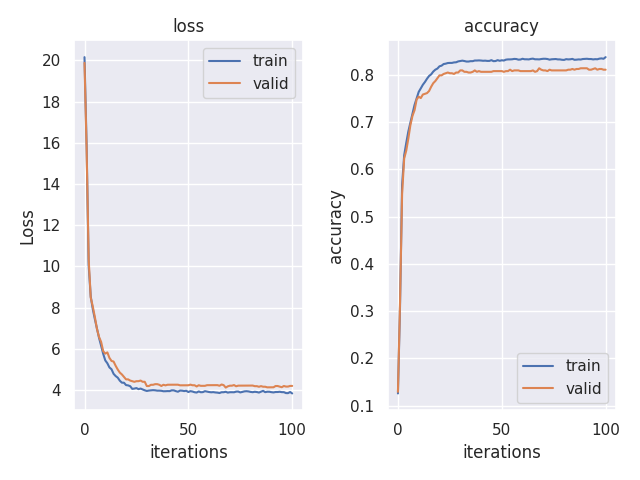
\includegraphics[width=\linewidth,height=5cm]{img/satlog-plots2}
	\captionof{figure}{Loss and accuracy during epochs for train and validation sets of Statlog.}
\end{center}

\begin{table*}[hbt]\centering
  \begin{tabular*}{1\textwidth}{@{\extracolsep{\fill} }ccccccccccc@{}}
		\toprule
		hidden\_layer & activation & epoch & eta & beta & alpha & mu & batch\_size & test\_score & train\_score & loss \\ \midrule
		(64,) & ReLu & 30 & 0.01 & 0.3 & 0.00 & 0.95 & 256 & 0.72 & 0.74 & 5.93 \\
		(64,) & Tanh & 30 & 0.01 & 0.2 & 0.00 & 0.95 & 256 & 0.71 & 0.74 & 6.19 \\
		(64,) & Tanh & 30 & 0.01 & 0.3 & 0.00 & 0.95 & 256 & 0.70 & 0.71 & 6.71 \\
		(64,) & ReLu & 30 & 0.01 & 0.2 & 0.01 & 0.95 & 256 & 0.68 & 0.70 & 7.39 \\
		(64,) & Sigmoid & 30 & 0.01 & 0.2 & 0.00 & 0.95 & 256 & 0.67 & 0.68 & 7.39 \\
		(64,) & ReLu & 30 & 0.01 & 0.2 & 0.00 & 0.95 & 256 & 0.66 & 0.68 & 7.38 \\
		(64,) & ReLu & 30 & 0.01 & 0.3 & 0.01 & 0.95 & 256 & 0.62 & 0.63 & 9.00 \\ \bottomrule
	\end{tabular*}
    \captionof{table}{Best architectures and corresponding scores for Statlog dataset}
    \label{tsatlog}
\end{table*}

\begin{figure*}\centering
	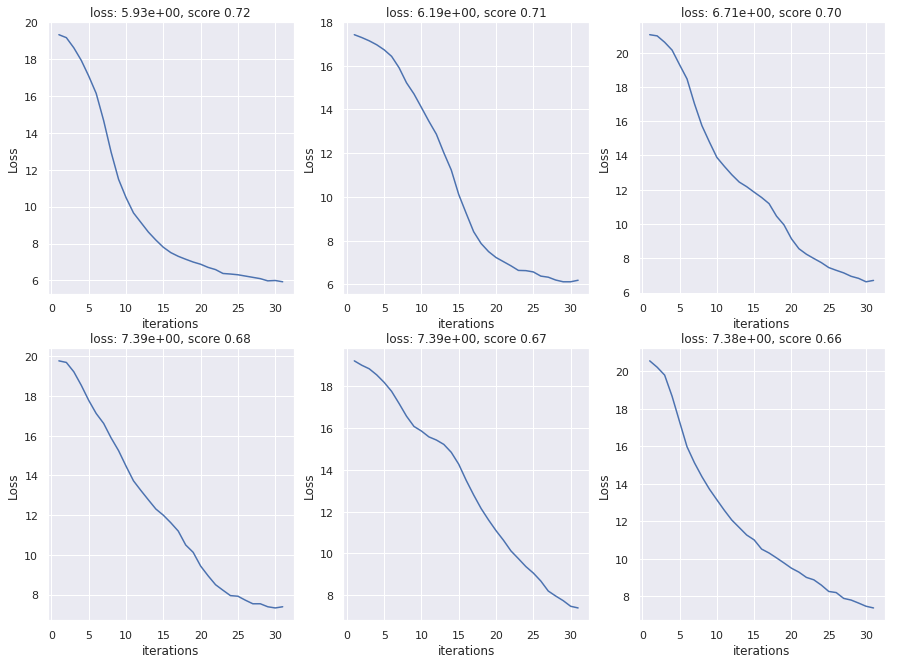
\includegraphics[width=1.79\columnwidth, height=10cm]{img/statlog-plots1}
	\caption{Loss value of best architectures for Statlog}
	\label{fsatlog}
\end{figure*}

\subsection{mnist}
The MNIST database of handwritten digits, available from this page, has a training set of 60,000 examples, and a test set of 10,000 examples. It is a subset of a larger set available from NIST. The digits have been size-normalized and centered in a fixed-size image. \href{http://yann.lecun.com/exdb/mnist/}{More information about mnist dataset is available on lecun.com.}
\\
The grid search parameters for this problem are set to

\begin{python}
hidden_layers = [(64,64),(128,64),
 (128, 32, 32),(128, 32, 32)]
activation=[ReLu(),LeakyReLu(.03)]
batch_size	s = [512]
epochs = [10]
mus = [0, .85]
betas = [.1,.2]
etas = [.001,.01]
alphas = [.001,0]
\end{python}
See the results in the table \ref{tmnist}. Again we trained a network with this architecture and reached the \textbf{87.91\%} accuracy on train set and \textbf{86.89\%} on test set in just 15 epochs.
\begin{python}
MLP([128, 64], activation=ReLu(),
batch_size=64, epochs=15, mu=0.85,
beta=.1, eta=.03, alpha=.001,
verbose=1, task='classification')
\end{python}
\begin{table*}[]
  \begin{tabular*}{1\textwidth}{@{\extracolsep{\fill} }ccccccccccc@{}}
		\toprule
		hidden\_layer & activation & epoch & eta & beta & alpha & mu & batch\_size & test\_score & train\_score & loss \\ \midrule
		(128, 64) & ReLu & 10 & 0.01 & 0.2 & 0.000 & 0.85 & 512 & 0.32 & 0.31 & 15.93 \\
		(128, 64) & LeakyReLu(0.03) & 10 & 0.01 & 0.2 & 0.000 & 0.85 & 512 & 0.29 & 0.28 & 16.58 \\
		(128,) & ReLu & 10 & 0.01 & 0.1 & 0.001 & 0.85 & 512 & 0.28 & 0.28 & 16.62 \\
		(128,) & ReLu & 10 & 0.01 & 0.1 & 0.000 & 0.85 & 512 & 0.28 & 0.27 & 16.73 \\
		(64, 64) & ReLu & 10 & 0.01 & 0.2 & 0.001 & 0.85 & 512 & 0.28 & 0.27 & 16.79 \\
		(128,) & LeakyReLu(0.03) & 10 & 0.01 & 0.1 & 0.000 & 0.85 & 512 & 0.27 & 0.28 & 16.67 \\ \bottomrule
	\end{tabular*}
	\caption{Best architectures and corresponding scores for MNIST dataset}
	\label{tmnist}
\end{table*}
\begin{figure*}\centering
	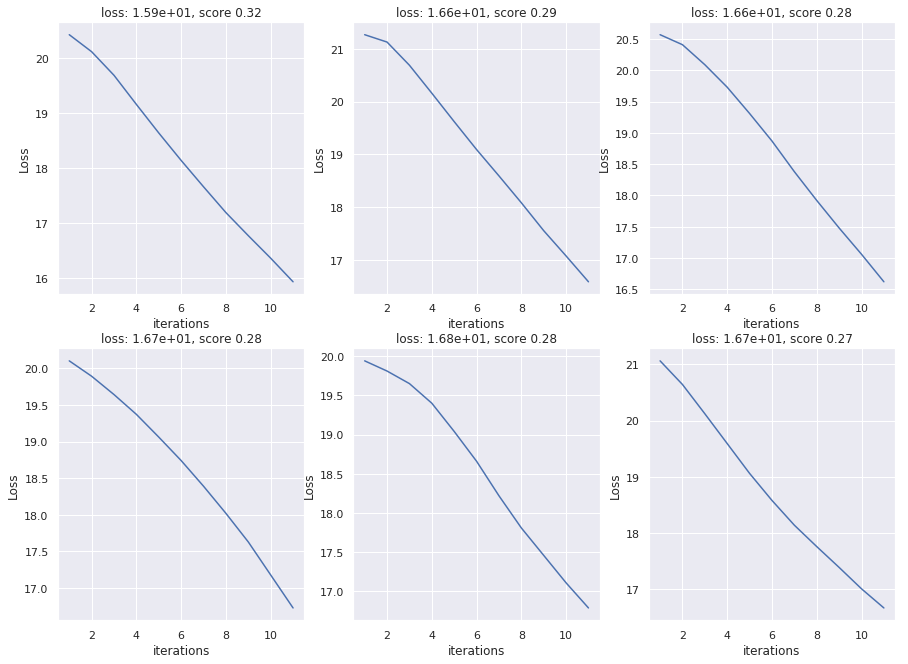
\includegraphics[width=1.79\columnwidth, height=10cm]{img/mnist-plots1}
	\caption{Loss value of best architectures for MNIST}
	\label{fmnist}
\end{figure*}
To reach this accuracy with just 15 epochs we reduced the batch size from 512 to 64. This shows the important role of batch size in training a netwrok. Another interesting fact we found is the effect of number of epochs on overfitting problen. In above figure, you sae that from iteration 7-8 the network validation accuracy is reducing.

\begin{center}
	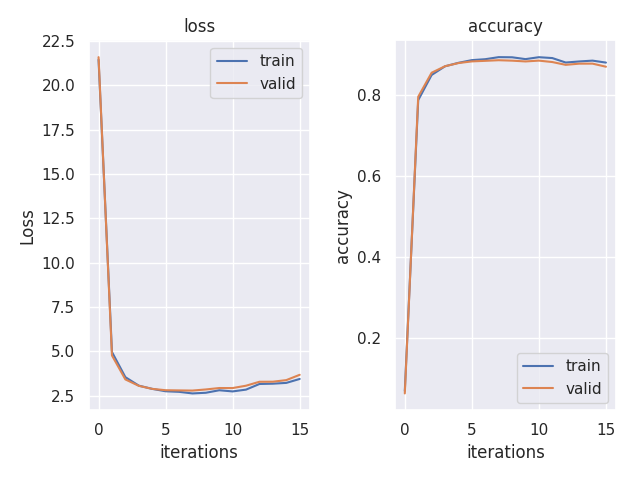
\includegraphics[width=1\linewidth,height=6cm]{img/mnist-plots2}
	\captionof{figure}{Loss and accuracy during epochs for train and validation sets of MNIST.}
	\label{fmnist2}
\end{center}


\subsection{Fashion mnist}
Fashion-MNIST is a dataset of Zalando's article images consisting of a training set of 60,000 examples and a test set of 10,000 examples. Each example is a 28x28 grayscale image, associated with a label from 10 classes. We intend Fashion-MNIST to serve as a direct drop-in replacement for the original MNIST dataset for benchmarking machine learning algorithms. It shares the same image size and structure of training and testing splits. \href{https://github.com/zalandoresearch/fashion-mnist}{More information in zalandoresearch's github repository.}

The grid search parameters are set to:
\begin{python}
hidden_layers = [(64,64),(128,64),
(128, 32, 32),(128, 32, 32)]
activation=[ReLu(),LeakyReLu(.03)]
batch_sizes = [512]
epochs = [10]
mus = [0, .85]
betas = [.1,.2]
etas = [.001,.01]
alphas = [.001,0]
\end{python}
\begin{table*}[]
  \begin{tabular*}{1\textwidth}{@{\extracolsep{\fill} }ccccccccccc@{}}
		\toprule
		hidden\_layer & activation & epoch & eta & beta & alpha & mu & batch\_size & test\_score & train\_score & loss \\ \midrule
		(128, 64) & LeakyReLu(0.03) & 10 & 0.01 & 0.2 & 0.001 & 0.85 & 512 & 0.48 & 0.48 & 12.04 \\
		(128, 64) & ReLu & 10 & 0.01 & 0.2 & 0.001 & 0.85 & 512 & 0.47 & 0.47 & 12.33 \\
		(128, 64) & ReLu & 10 & 0.01 & 0.2 & 0.000 & 0.85 & 512 & 0.47 & 0.47 & 12.22 \\
		(128, 64) & LeakyReLu(0.03) & 10 & 0.01 & 0.2 & 0.000 & 0.85 & 512 & 0.45 & 0.45 & 12.60 \\
		(64, 64) & LeakyReLu(0.03) & 10 & 0.01 & 0.2 & 0.001 & 0.85 & 512 & 0.42 & 0.42 & 13.48 \\
		(128, 32, 32) & ReLu & 10 & 0.01 & 0.2 & 0.000 & 0.85 & 512 & 0.39 & 0.40 & 13.84 \\ \bottomrule
	\end{tabular*}
\caption{Best architectures and corresponding scores for Fashion MNIST dataset}
\label{tfashion}
\end{table*}
\begin{figure*}\centering
	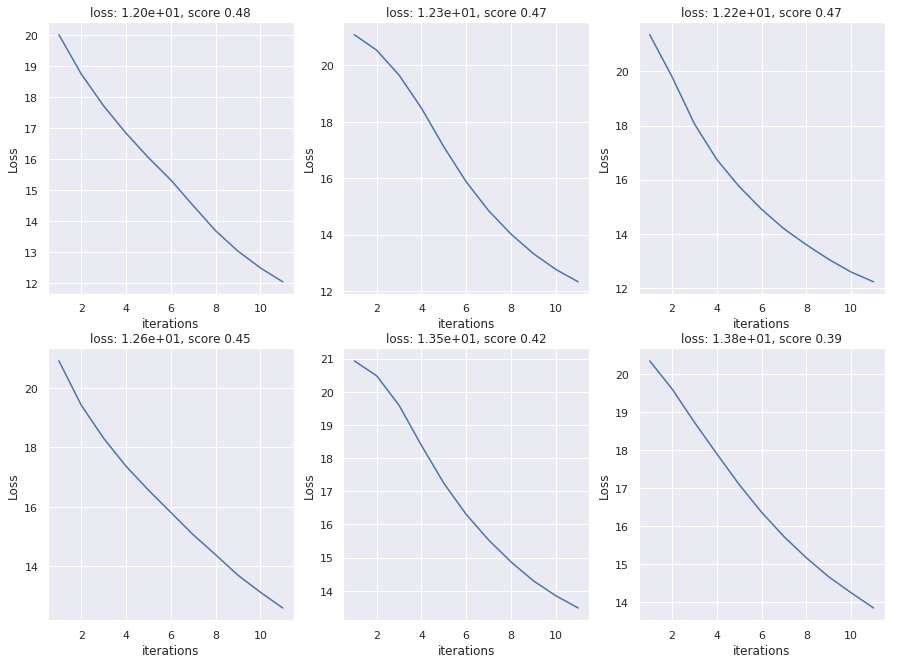
\includegraphics[width=1.79\columnwidth, height=10cm]{img/fashion-plots1}
	\caption{Loss value of best architectures for Fashion mnist}
	\label{ffashion}
\end{figure*}
Again we trained a network with this architecture and reached the \textbf{76.78\%} accuracy on train set and \textbf{75.36\%} on test set in just 10 epochs.
\\
\\
\begin{python}
MLP([128, 64], mu=0.85,
activation=LeakyReLu(.03),
batch_size=64, epochs=10, 
beta=.2, eta=.01, alpha=.001,
verbose=1, task='classification')
\end{python}
\begin{center}
	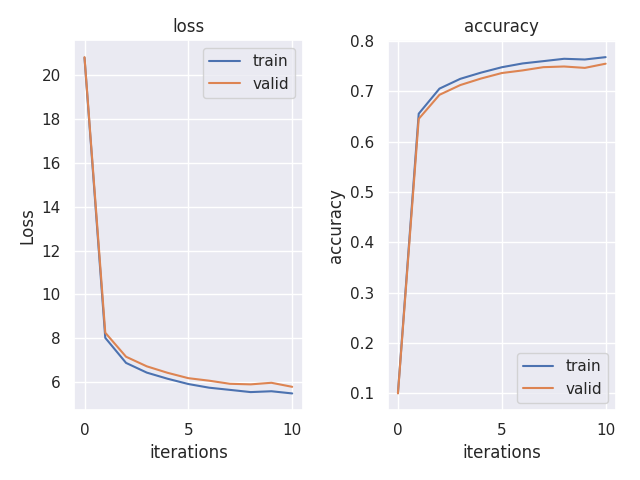
\includegraphics[width=\linewidth,height=6cm]{img/fashion-plots2}
	\captionof{figure}{Loss and accuracy during epochs for train and validation sets of Fashion MNIST.}
	\label{ffashion2}
\end{center}
The above figures shows that, unlike iris dataset, the validation accuracy is always lower that training accuracy. 

To increase the accuracy, we changed the model from MLP to CNN and tested different architectures on this dataset.\\

\textbf{Test 1)}  For the first test case we used a single convolution layer connected to a fully connected layer with 10 neurons and softmax activation function which classifies the input of the network. To show the effect of the convolution layer hyperparameters, we evaluated the network on five different feature maps $\{8,16,32,64,128\}$, five different kernel sizes $\{3\times3, 5\times5, 7\times7,9\times9,11\times11\}$ and two different padding strategies \{same, valid\} for grid search parameters with relu activation function, keras default Adam optimizer, batch size 256 and 10 epochs. Table \ref{tfashion1} shows the best result of these models. Although different kernel size and number of filters is used to reach better accuracy, all of the results used only $same$ padding. 
\\
\textbf{Test 2)} In the table \ref{tfashion2} we extended this architecture with 2 convolutional layers. The results shows that by increasing the network depth, $3\times3$ kernel size performs better than bigger kernels.
\\
\textbf{Test 3)} In this experiment we increased the convolutional layers and epochs to 3 and 20, respectively. Also we reduced batch size to 128. See table \ref{tfashion3}. In this table even the train accuracy reached to 100\% but test score is same as previous examples. To overcome this issue we added a Dense layer with 32 neurons after last convolutional layer. See table  \ref{tfashion4}. In the table \ref{tfashion5} we changed filter sizes. These tables shows that increasing the number of filters instead of setting a fixed feature map, can perform better. All of the examples, used smaller kernel sizes. So for next examples we use $3\times3$ kernel sizes along with increasing filter sizes trough depth of network.

\subsection{Cifar10}
The CIFAR-10 dataset contains 60,000 32x32 color images in 10 different classes. The 10 different classes represent airplanes, cars, birds, cats, deer, dogs, frogs, horses, ships, and trucks. There are 6,000 images of each class. To show the effect of batch normalization effect on the dataset, we designed this architecture for cifar10 classification
\\
\begin{python}
[Conv2D(32, (3, 3),padding='same',
       activation='relu'),
Conv2D(64, (3, 3),padding='same',
       activation='relu'),
Conv2D(128, (3, 3),padding='same',
       activation='relu'),
Flatten(),
Dense(256, activation='relu'),
Dense(128, activation='relu'),
Dense(10, activation='softmax')]
\end{python}
and ran the model with 10 epochs of adam optimizer and batch size 128. Without the normalization the accuracy of model on test set was $10\%$ but when we added this layer, the accuracy became $64.4\%$. This model has $33,682,134$ parameters which should be trained using adam optimizer. Here by adding three pooling layers we construct this model 
\begin{python}
[Conv2D(32, (3, 3),padding='same',
      activation='relu'),
MaxPooling2D((2,2)),
Conv2D(64, (3, 3),padding='same',
     activation='relu'),
MaxPooling2D((2,2)),
Conv2D(128, (3, 3),padding='same',
     activation='relu'),
MaxPooling2D((2,2)),
Flatten(),
Dense(256, activation='relu'),
Dense(128, activation='relu'),
Dense(10, activation='softmax')]
\end{python}
Although this model has just $651,990$ parameters the accuracy became $74.6\%$ on the test set and $93\%$ on train set which is a big achievement in both accuracy and speed. In this example we saw a little overfitting on the model since the difference between accuracy is about $18\%$. Here by add two dropout layers we reduced overfitting to about $8\%$. The new architecture is as follows
\begin{python}
[Conv2D(32, (3, 3),padding='same',
      activation='relu'),
Dropout(.5),
MaxPooling2D((2,2)),
Conv2D(64, (3, 3),padding='same',
     activation='relu'),
MaxPooling2D((2,2)),
Conv2D(128, (3, 3),padding='same',
     activation='relu'),
MaxPooling2D((2,2)),
Flatten(),
Dense(256, activation='relu'),
Dropout(.5),
Dense(128, activation='relu'),
Dense(10, activation='softmax')]
\end{python}
To show the effect of optimizer algorithm in the classification task when all of other hyperparameters are fixed, we changed the optimizer from adam to rmsprop and sgd and saw that the accuracy decreased from $72.5\%$ to $72.2$ and $60.5\%$, respectively. 
For the last try, we changed the learning rate parameter of adam  to show the effect of learning rate to the accuracy.  See results in the table \ref{tadams}.
\begin{center}
	\begin{tabular*}{.85\linewidth}{@{\extracolsep{\fill} }ccc@{}}
		\toprule
learning rate & epochs &accuracy \\ \midrule
1e-1&10 & 10\% \\
1e-2&10 & 42\% \\
1e-3 &10& 74\% \\
1e-4 &10& 64\% \\ 

1e-1 &50 & 10\% \\
1e-2 &50 & 47.4\% \\
1e-3 &50& 74.8\% \\
1e-4 &50& 72.8\% \\ 
\bottomrule
	\end{tabular*}
	\captionof{table}{The effect of epochs and learning for adam optimizer on cifar10 test set}
	\label{tadams}
\end{center}

\subsection{Sentiment analysis}

See dataset info in \href{https://www.kaggle.com/ashukr/rnnsentiment-data}{kaggle}. We splitted the data set into 67\% train and 33\% test set. The first test case in this example consist of 108 tries, with 12 different architectures and 9 different permutations of sentence configuration. To do this we first preprocess the documents and convert sentences to a sequence of integers. To apply this sequence into network we should align all sequences to a fixed size length. We tested 3 different lengths $100,200,500$. Since some words in the documents are appear frequently we removed 15 top common words from the sequences. Then fed this fixed size sequences to an embedding layer with $10,50,100,200$ output dimension along with one LSTM cell of $8,16,64$ units. Table \ref{tsentiment1} shows the accuracy of these models. All of the results obtained by just 5 epochs of Keras default Adam optimizer with batch size 256.  As the second try, we designed a more complex network consist of en embedding layer followed by two LSTM cells. Table \ref{tsentiment2} shows the results of this experiment ran in 15 epochs. Also in this example we used Bidirectional LSTM architecture to see the effect of this layer, but doesn't affect the accuracy.  For the last try, we designed a convolutional-LSTM network. This model performs better that previous models and reached $82\%$ accuracy. Note that the first layer of this model is an embedding layer with output\_dim=200, input\_dim=715 and input\_length=100. Here is the code of proposed architecture in presented library.
\begin{python}
N=max_dict_words + skip_common
[Embedding(N, 200, input_length=
max_sent_words), 
LSTM(16, return_sequences=True),
Conv1D(16, 3, padding='valid',
activation='relu', strides=1),
GlobalMaxPooling1D(),
Dense(16,activation='relu'),
Dense(2, activation='softmax')]
\end{python}
\section{Concluding remarks}
In this exercise, we implemented a simple multi layer perceptron neural network from scratch with matrix form formulations which is very important where the number of neurons and layers are large. Our implementation is appropriate for both regression and classification tasks by just setting an argument. All of the preprocessing requirements such as scaling and encoding are done by $MLP$ class automatically. To tune the hyperparametes of the network for a specific dataset, we implemented a $MLPGridSearch$ class which uses $parallelization$ techniques and finds optimal architecture among all possible solutions. In the second part of the report, we implemented a $CNN$ class based on awesome $keras$ module which is based on $tensorflow$ a scientific computation package. Also to find optimal architecture, we implemented a $CNNGridSearch$ class with the same interface of $MLPGridSearch$ class. The third part, implements $RNN$ based networks with an interface similar to $CNN$. Again to optimize the network architecture, we implemented $RNNGridSearch$. We tested this networks on 6 different datasets which is used by many researchers for classification tasks. The results shows the important role of model type and architecture, batch size, number of epochs, activation function and learning rate for training a network. Also to prevent overfitting problem we saw the effect of dropout layer in the networks. 

\begin{table*}[]
	\begin{tabular*}{1\linewidth}{@{\extracolsep{\fill} }lccc@{}}
		\toprule
		architecture & test & train & loss \\ \midrule
		Conv(filters=128, kernel=(11, 11)) & 0.88 & 0.93 & 0.19 \\
		Conv(filters=64, kernel=(5, 5)) & 0.87 & 0.95 & 0.15 \\
		Conv(filters=128, kernel=(5, 5)) & 0.87 & 0.95 & 0.14 \\
		Conv(filters=32, kernel=(7, 7)) & 0.87 & 0.94 & 0.16 \\
		Conv(filters=32, kernel=(9, 9)) & 0.87 & 0.93 & 0.18 \\
		Conv(filters=64, kernel=(9, 9)) & 0.87 & 0.93 & 0.20 \\ \bottomrule
	\end{tabular*}
	\caption{Train and test score for fashion mnist CNN  with different configurations}
	\label{tfashion1}
\end{table*}

\begin{table*}[]
	\begin{tabular*}{1\linewidth}{@{\extracolsep{\fill} }lccc@{}}
		\toprule
		architecture & test & train & loss \\ \midrule
		Conv(filters=32, kernel=(3, 3)),Conv(filters=32, kernel=(3, 3)) & 0.88 & 0.96 & 0.11 \\
		Conv(filters=32, kernel=(7, 7)),Conv(filters=32, kernel=(7, 7)) & 0.88 & 0.95 & 0.14 \\
		Conv(filters=16, kernel=(11, 11)),Conv(filters=16, kernel=(11, 11)) & 0.88 & 0.93 & 0.18 \\
		Conv(filters=128, kernel=(7, 7)),Conv(filters=128, kernel=(7, 7)) & 0.86 & 0.95 & 0.15 \\
		Conv(filters=64, kernel=(11, 11)),Conv(filters=64, kernel=(11, 11)) & 0.86 & 0.95 & 0.14 \\
		Conv(filters=16, kernel=(7, 7)),Conv(filters=16, kernel=(7, 7)) & 0.86 & 0.94 & 0.16 \\ \bottomrule
	\end{tabular*}
	\caption{Train and test score for fashion mnist CNN  with different configurations}
	\label{tfashion2}
\end{table*}

\begin{table*}[]
	\begin{tabular*}{1\linewidth}{@{\extracolsep{\fill} }lccc@{}}
		\toprule
		architecture & test & train & loss \\ \midrule
		Conv(filters=16, kernel=(3, 3)),Conv(filters=16, kernel=(3, 3)),Conv(filters=16, kernel=(3, 3)) & 0.84 & 0.99 & 0.04 \\
		Conv(filters=32, kernel=(7, 7)),Conv(filters=32, kernel=(7, 7)),Conv(filters=32, kernel=(7, 7)) & 0.82 & 0.98 & 0.04 \\
		Conv(filters=32, kernel=(7, 7)),Conv(filters=32, kernel=(7, 7)),Conv(filters=32, kernel=(7, 7)) & 0.82 & 0.98 & 0.06 \\
		Conv(filters=16, kernel=(3, 3)),Conv(filters=16, kernel=(3, 3)),Conv(filters=16, kernel=(3, 3)) & 0.80 & 0.99 & 0.03 \\ \bottomrule
	\end{tabular*}
	\caption{Train and test score for fashion mnist CNN  with different configurations}
	\label{tfashion3}
\end{table*}
\begin{table*}[]
	\begin{tabular*}{1\linewidth}{@{\extracolsep{\fill} }lcc@{}}
		\toprule
		architecture & test & train \\ \midrule
		Conv(filters=16, kernel=(3,3)),Conv(filters=16, kernel=(3, 3)),Conv(filters=16, kernel=(3,3)),Dense(units=32) & 0.86 & 0.99  \\
		Conv(filters=16, kernel=(3,3)),Conv(filters=16, kernel=(3, 3)),Conv(filters=16, kernel=(3,3)),Dense(units=32) & 0.85 & 1.00  \\
		Conv(filters=32, kernel=(7,7)),Conv(filters=32, kernel=(7, 7)),Conv(filters=32, kernel=(7,7)),Dense(units=32) & 0.84 & 0.99 \\
		Conv(filters=32, kernel=(7,7)),Conv(filters=32, kernel=(7, 7)),Conv(filters=32, kernel=(7,7)),Dense(units=32) & 0.83 & 0.99 \\ \bottomrule
	\end{tabular*}
	\caption{Train and test score for fashion mnist CNN  with different configurations}
	\label{tfashion4}
\end{table*}
\begin{table*}[]
	\begin{tabular*}{1\linewidth}{@{\extracolsep{\fill} }lcc@{}}
		\toprule
		architecture & test & train  \\ \midrule
		Conv(filters=8, kernel=(3, 3)),Conv(filters=16, kernel=(3, 3)),Conv(filters=32, kernel=(3, 3)),Dense(units=32) & 0.89 & 1.00 \\
		Conv(filters=8, kernel=(7, 7)),Conv(filters=16, kernel=(7, 7)),Conv(filters=32, kernel=(7, 7)),Dense(units=32) & 0.86 & 0.99 \\
		Conv(filters=8, kernel=(3, 3)),Conv(filters=16, kernel=(3, 3)),Conv(filters=32, kernel=(3, 3)),Dense(units=32) & 0.85 & 1.00  \\
		Conv(filters=8, kernel=(7, 7)),Conv(filters=16, kernel=(7, 7)),Conv(filters=32, kernel=(7, 7)),Dense(units=32) & 0.85 & 0.99  \\ \bottomrule
	\end{tabular*}
	\caption{Train and test score for fashion mnist CNN  with different configurations}
	\label{tfashion5}
\end{table*}

\begin{table*}[]
	\begin{tabular*}{1\linewidth}{@{\extracolsep{\fill} }lccc@{}}
		\toprule
		architecture & test\_score & train\_score & loss \\ \midrule
		Embedding(output\_dim=200, input\_dim=515, input\_length=100),LSTM(units=64) & 0.814 & 0.840 & 0.35 \\
		Embedding(output\_dim=200, input\_dim=515, input\_length=100),LSTM(units=8) & 0.811 & 0.840 & 0.36 \\
		Embedding(output\_dim=100, input\_dim=515, input\_length=100),LSTM(units=16) & 0.809 & 0.840 & 0.35 \\
		Embedding(output\_dim=200, input\_dim=515, input\_length=100),LSTM(units=16) & 0.809 & 0.840 & 0.35 \\
		Embedding(output\_dim=50, input\_dim=515, input\_length=100),LSTM(units=64) & 0.806 & 0.830 & 0.39 \\ \bottomrule
	\end{tabular*}
	\caption{Train and test score for sentiment analysis with different configurations}
\label{tsentiment1}
\end{table*}

\begin{table*}[]
	\begin{tabular*}{1\linewidth}{@{\extracolsep{\fill} }lcc@{}}
		\toprule
		architecture & test & train \\ \midrule
		Embedding(output\_dim=200, input\_dim=725, input\_length=100),LSTM(units=32) & 0.799 & 0.870 \\
		Embedding(output\_dim=200, input\_dim=725, input\_length=100),LSTM(units=32) & 0.796 & 0.920 \\
		Embedding(output\_dim=500, input\_dim=725, input\_length=100),LSTM(units=32),LSTM(units=32) & 0.795 & 0.950 \\
		Embedding(output\_dim=1000, input\_dim=725, input\_length=100),LSTM(units=32) & 0.795 & 0.930 \\ \bottomrule
	\end{tabular*}
\caption{Train and test score for sentiment analysis with different configurations}
\label{tsentiment2}
\end{table*}
\begin{table*}[t!]
	\begin{tabular*}{1\linewidth}{@{\extracolsep{\fill} }lcc@{}}
		\toprule
		architecture & test\_score & train\_score \\ \midrule
		LSTM(units=16),Conv1D(kernel=(3,), filters=16),GlobalMaxPooling1D(),Dense(units=16) & 0.820 & 0.880 \\
		LSTM(units=16),Conv1D(kernel=(3,), filters=8),GlobalMaxPooling1D(),Dense(units=16) & 0.818 & 0.880 \\
	LSTM(units=16),Conv1D(kernel=(5,), filters=8),GlobalMaxPooling1D(),Dense(units=16) & 0.812 & 0.880 \\
		Conv1D(kernel=(3,), filters=16),GlobalMaxPooling1D(),Dense(units=16) & 0.806 & 0.940 \\
		\multicolumn{1}{l}{} &  &  \\ \bottomrule
	\end{tabular*}
\caption{Train and test score for sentiment analysis with different configurations}
\label{tsentiment3}
\end{table*}
\end{document}